\chapter{Von Teilchen zu einem einfachen Quantenfeld}

Bauen wir das einfache Quantenfeld noch einmal auf, diesmal jedoch aus einem etwas anderen Blickwinkel. Es gibt zwei Wege zur Quantenfeldtheorie. Wir können von Teilchen ausgehen und herausfinden, warum ein Feld ihre natürliche Beschreibungssprache ist, oder mit einem Wellenfeld beginnen und untersuchen, warum seine Anregungen in Quanten auftreten. Beide Wege sind nützlich. Hier folgen wir dem ersten.

Die gewöhnliche Quantenmechanik kann ein Teilchen, zwei Teilchen oder eine andere festgelegte Teilchenzahl beschreiben. Die Natur hält sich nicht an diese Einschränkung. Die Zahl der Photonen in einem Raum ändert sich, wenn die Lampen Strahlung aussenden oder absorbieren. Instabile Teilchen zerfallen. Beim Betazerfall beispielsweise gilt
\begin{equation}
n\longrightarrow p+e^-+\bar{\nu}_e,
\end{equation}
sodass sich die Besetzungszahlen mehrerer Teilchensorten zugleich ändern. Wir benötigen daher eine Quantenmechanik, die groß genug ist, um alle möglichen Besetzungszahlen und schließlich auch Prozesse zu umfassen, die zwischen ihnen wechseln.

Vorerst vereinfachen wir das Problem stark. Es gibt nur eine Sorte nichtrelativistischer Teilchen. Zunächst erweitern wir den Zustandsraum so, dass er jede Teilchenzahl aufnehmen kann; erst danach behandeln wir mehrere Sorten, Relativität, Streuung und Zerfall. Die Mathematik ist nicht besonders schwierig, doch der Perspektivwechsel ist abstrakt. Es lohnt sich, die Schritte langsam genug zu gehen, damit die Notation die Idee nicht verdeckt.

\section{Der Ausgangspunkt: ein Teilchen}

Wir beginnen mit einem einzelnen Teilchen im Zustand \(|\psi\rangle\). Seine Ortsraum-Wellenfunktion lautet
\begin{equation}
\psi(x)=\langle x|\psi\rangle.
\label{eq:l07-wavefunction}
\end{equation}
Dieses kleingeschriebene \(\psi\) ist eine gewöhnliche komplexwertige Funktion. Es ist noch kein Quantenfeld und auch kein Operator auf einem Vielteilchen-Zustandsraum.

Die Bornsche Regel besagt, dass
\begin{equation}
\rho_\psi(x)=|\psi(x)|^2=\psi^*(x)\psi(x)
\label{eq:l07-born-density}
\end{equation}
die Wahrscheinlichkeitsdichte dafür ist, das Teilchen bei \(x\) zu finden. Für einen normierten Zustand gilt
\begin{equation}
\int dx\,\psi^*(x)\psi(x)=1.
\label{eq:l07-one-particle-normalization}
\end{equation}
Die rechte Seite ist die Gesamtwahrscheinlichkeit. Da dieses Problem genau ein Teilchen enthält, entspricht sie zugleich der Teilchenzahl. Dieser Gleichklang wird sich als nützlicher Hinweis erweisen, ist hier jedoch trivial.

\begin{classroomqa}
\lecturetimestamp{00:09:13}
\audiencequestion{Warum muss die Wahrscheinlichkeitsdichte die Form \(\psi^*(x)\psi(x)\) haben?}
\lecturerresponse{Das ist die Bornsche Regel, eines der Postulate der Quantenmechanik. Die Amplitude für das Messergebnis „Ort“ \(x\) ist \(\langle x|\psi\rangle\); die Wahrscheinlichkeitsdichte ist ihr Betragsquadrat. Sie wird nicht aus der später verwendeten Feldkonstruktion hergeleitet.}
\end{classroomqa}

\enlargethispage{1pt}
\section{Moden, Orthogonalität und Vollständigkeit}

Für den Einteilchen-Hilbertraum gibt es viele nützliche Basen. Die Orts-Eigenzustände bilden eine Basis. Auch die Eigenzustände eines beliebigen hermiteschen Operators bilden eine, unter den üblichen Vorbehalten bei Entartungen und kontinuierlichen Spektren. Da die Energie bald wichtig wird, wählen wir ein vollständiges Orthonormalsystem von Energie-Eigenzuständen eines Teilchens:
\begin{equation}
|1\rangle,\ |2\rangle,\ldots,
\qquad
\psi_i(x)=\langle x|i\rangle.
\end{equation}

Beim Teilchen im Kasten wird der Index \(i\) anschaulich. Die Wellenfunktion des Grundzustands hat keinen inneren Knoten, die des nächsten Zustands einen, und die höheren Zustände schwingen immer schneller. In einem idealen unendlich tiefen Potentialtopf sind es im Wesentlichen Sinuswellen.

\begin{figure}[htbp]
\centering
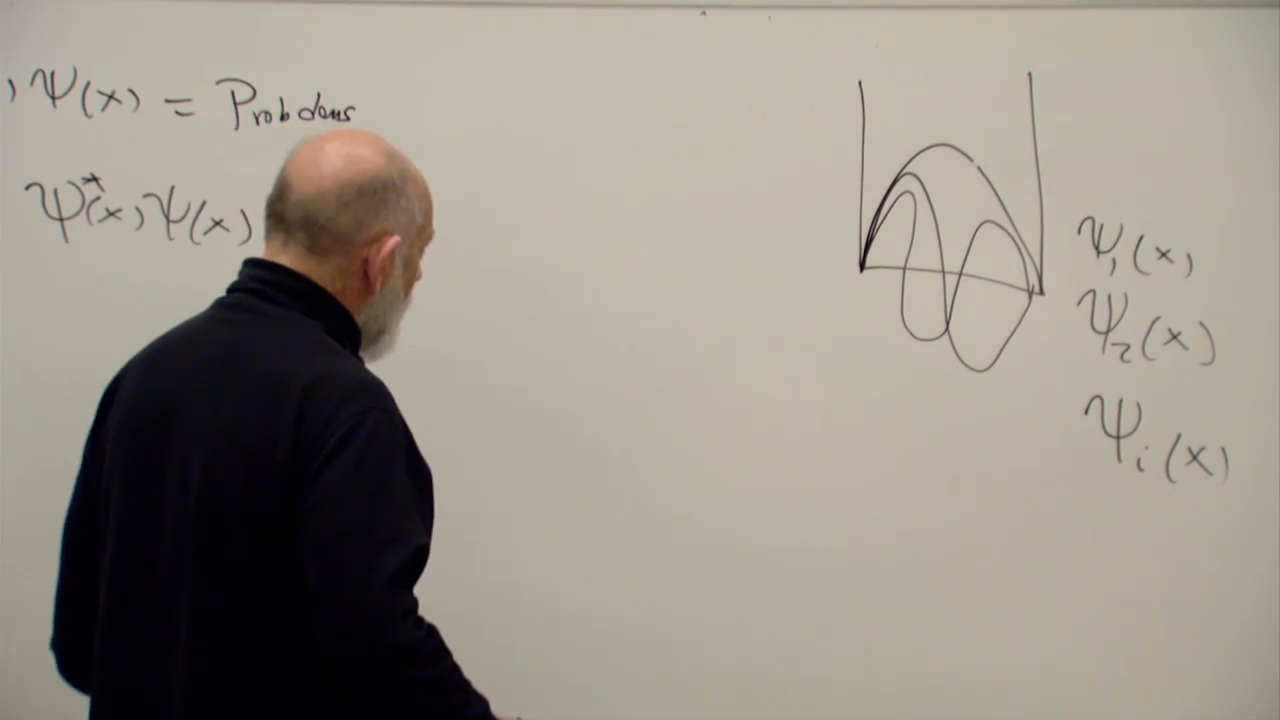
\includegraphics[width=0.94\linewidth]{lecture_07_frame_01.png}
\caption{Die Kastenmoden an der Vorlesungstafel. Links sind noch die Bornsche Einteilchen-Wahrscheinlichkeitsdichte und die Normierung zu sehen; der Potentialtopf rechts zeigt \(\psi_1(x)\), \(\psi_2(x)\) und die allgemeine Bezeichnung \(\psi_i(x)\).}
\lectureframe{00:08:25}
\end{figure}

Dieselbe Modenstruktur lässt sich auch unabhängig von der Überdeckung durch die Live-Tafel darstellen:
\begin{figure}[htbp]
\centering
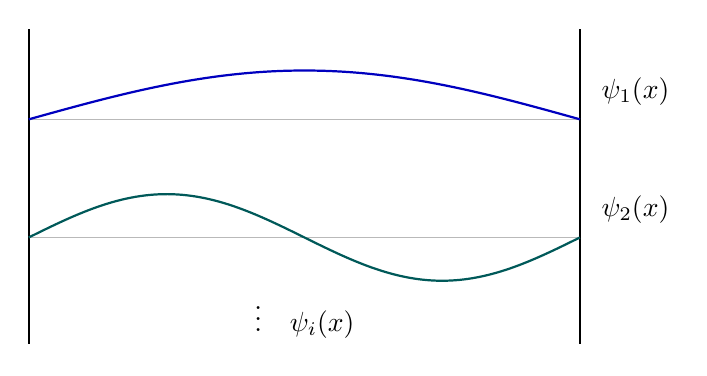
\begin{tikzpicture}[x=1cm,y=1cm]
  \draw[thick] (0,0) -- (0,4.0);
  \draw[thick] (7,0) -- (7,4.0);
  \draw[gray!55] (0,2.85) -- (7,2.85);
  \draw[gray!55] (0,1.35) -- (7,1.35);
  \draw[blue!75!black,thick,domain=0:7,samples=120]
    plot (\x,{2.85+0.62*sin(180*\x/7)});
  \draw[teal!70!black,thick,domain=0:7,samples=120]
    plot (\x,{1.35+0.55*sin(360*\x/7)});
  \node[right] at (7.15,3.20) {$\psi_1(x)$};
  \node[right] at (7.15,1.70) {$\psi_2(x)$};
  \node at (3.5,0.38) {$\vdots\quad\psi_i(x)$};
\end{tikzpicture}
\caption{Eine saubere Rekonstruktion der qualitativen Kastenskizze. Die vertikalen Verschiebungen dienen lediglich dazu, die beiden Wellenfunktionen in der Darstellung voneinander zu trennen.}
\end{figure}

Die Orthonormalitätsbedingung lautet
\begin{equation}
\int dx\,\psi_i^*(x)\psi_j(x)=\delta_{ij}.
\label{eq:l07-orthonormality}
\end{equation}
Für \(i=j\) ist der Zustand normiert und das Integral gleich eins. Für \(i\ne j\) sind die beiden Zustände orthogonal und das Integral verschwindet.

Vollständigkeit ist die ebenso wichtige Aussage
\begin{equation}
\sum_i |i\rangle\langle i|=\mathbf 1.
\label{eq:l07-resolution}
\end{equation}
Jedes \(|i\rangle\langle i|\) projiziert auf eine Basisrichtung; die Summe über die vollständige Basis ist die Einheitsabbildung. Auf einen beliebigen Vektor angewandt, zerlegt sie ihn lediglich in seine Komponenten und setzt ihn wieder zusammen.

Nun schieben wir Gleichung~\eqref{eq:l07-resolution} zwischen zwei Ortszustände:
\begin{align}
\langle y|x\rangle
&=\sum_i\langle y|i\rangle\langle i|x\rangle \\
&=\sum_i\psi_i(y)\psi_i^*(x) \\
&=\delta(y-x).
\label{eq:l07-position-completeness}
\end{align}
Der Stern gehört an den Faktor, dessen Bra-Ket-Reihenfolge \(\langle i|x\rangle\) lautet. Vertauscht man \(x\) und \(y\), erhält man die komplex konjugierte, aber gleichwertige Form. Jede vollständige Orthonormalbasis liefert somit eine Darstellung der Deltafunktion. Sinus- und Kosinusfunktionen, Oszillator-Wellenfunktionen und Energie-Eigenfunktionen erfüllen alle dieselbe Aufgabe.

\begin{classroomqa}
\lecturetimestamp{00:13:43}
\audiencequestion{Muss die zweite Wellenfunktion in der Vollständigkeitssumme komplex konjugiert werden?}
\lecturerresponse{Ja. Bei der Reihenfolge \(\langle y|i\rangle\langle i|x\rangle\) lauten die Faktoren \(\psi_i(y)\psi_i^*(x)\). Wenn man die Bra-Ket-Reihenfolge sichtbar lässt, muss man nicht raten, wo der Stern hingehört.}
\end{classroomqa}

Das ist die Einteilchen-Mathematik, die wir benötigen. Nun wechseln wir den Zustandsraum.

\section{Der Fockraum als erweiterter Zustandsraum}

Für viele identische Teilchen ist eine Basis praktisch, die angibt, wie viele Teilchen jede Einteilchenmode besetzen:
\begin{equation}
|n_1,n_2,n_3,\ldots\rangle.
\label{eq:l07-fock-basis}
\end{equation}
Die ganze Zahl \(n_i\) ist die Besetzungszahl der Mode \(i\). Dieser Ket ist kein Einteilchenzustand in ausgefallener Schreibweise. Er gehört zu einem größeren Hilbertraum, der den Nullteilchensektor, sämtliche Einteilchenzustände, sämtliche Zweiteilchenzustände und so weiter enthält. Dieser größere Raum heißt Fockraum.

Um Besetzungen zu ändern, führen wir für jede Mode einen Erzeugungsoperator und einen Vernichtungsoperator ein:
\begin{equation}
a_i^\dagger,\qquad a_i.
\end{equation}
Der erste fügt der Mode \(i\) ein Teilchen hinzu, der zweite entfernt eines. Die Sprache des harmonischen Oszillators dient hier zunächst als Buchführungshilfe: Es muss keine tatsächliche Feder schwingen. Die Oszillatoralgebra liefert genau die Werkzeuge, die wir benötigen, um Besetzungszahlen zu erhöhen und zu verringern.

Der Besetzungszahloperator der Mode ist
\begin{equation}
\begin{aligned}
N_i&=a_i^\dagger a_i,\\
N_i|n_1,\ldots,n_i,\ldots\rangle
&=n_i|n_1,\ldots,n_i,\ldots\rangle.
\end{aligned}
\end{equation}
Das Vakuum ist
\begin{equation}
|0\rangle\equiv|0,0,0,\ldots\rangle,
\qquad
a_i|0\rangle=0
\quad\text{for every }i.
\label{eq:l07-vacuum}
\end{equation}
Ein Einteilchenzustand in der Mode \(i\) ist daher
\begin{equation}
|i\rangle=a_i^\dagger|0\rangle.
\label{eq:l07-mode-created}
\end{equation}
Dasselbe Symbol \(|i\rangle\) kann nun entweder als Einteilchenbasisvektor oder als dieser Vektor aufgefasst werden, eingebettet in den Einteilchensektor des Fockraums. Die Einbettung ist Gleichung~\eqref{eq:l07-mode-created}; aus dem jeweiligen Kontext geht hervor, welcher Raum gemeint ist.

\section{Die Moden zu einem Feld zusammenfassen}

Wir definieren das Vernichtungsfeld und das Erzeugungsfeld durch
\begin{equation}
\Psi(x)=\sum_i \psi_i(x)a_i,
\qquad
\Psi^\dagger(x)=\sum_i \psi_i^*(x)a_i^\dagger.
\label{eq:l07-field-expansion}
\end{equation}
Die Großschreibung ist wichtig. Die kleingeschriebenen Funktionen \(\psi_i(x)\) sind komplexe Zahlen; das großgeschriebene \(\Psi(x)\) ist ein Operator auf dem Fockraum. Für jeden Raumpunkt \(x\) ergibt Gleichung~\eqref{eq:l07-field-expansion} eine andere Linearkombination der Modenoperatoren. Das bedeutet es, wenn man von einer operatorwertigen Funktion des Ortes spricht.

Bei freien Teilchen können die Modenfunktionen ebene Wellen \(e^{ikx}\) sein. Dann ist Gleichung~\eqref{eq:l07-field-expansion} eine Fourierentwicklung, nur dass ihre Fourierkoeffizienten Operatoren statt Zahlen sind. In der älteren Terminologie heißen gewöhnliche komplexe Zahlen \(c\)-Zahlen und Quantenoperatoren \(q\)-Zahlen. Die Modenfunktionen sind \(c\)-Zahlen und kommutieren mit allem; \(a_i\) und \(a_i^\dagger\) tragen den Operatorcharakter.

Weder \(\Psi\) noch \(\Psi^\dagger\) ist hermitesch. Ihre adjungierten Operatoren sind jeweils der andere. Die beiden Kombinationen
\begin{equation}
\Psi+\Psi^\dagger,
\qquad
i(\Psi^\dagger-\Psi)
\label{eq:l07-hermitian-combinations}
\end{equation}
sind hermitesch und können Observablen darstellen. Vorerst sind die Felder jedoch vor allem nützlich, um Teilchen lokal zu erzeugen, zu vernichten und zu zählen.

\begin{classroomqa}
\lecturetimestamp{00:21:05}
\audiencequestion{Was bedeutet es, dass ein Operator von \(x\) abhängt?}
\lecturerresponse{Das bedeutet, dass jeder Wert von \(x\) einen anderen Operator auswählt. Die Ortsabhängigkeit steckt in den gewöhnlichen Modenfunktionen, während jede daraus entstehende Linearkombination auf denselben Fockraum wirkt.}
\end{classroomqa}

\section{Was das Erzeugungsfeld bewirkt}

Eine Definition wird nützlich, wenn wir fragen, was sie bewirkt. Wir beginnen mit einem Orts-Eigenzustand im Einteilchensektor und setzen die Vollständigkeitsrelation ein:
\begin{align}
|x\rangle
&=\sum_i |i\rangle\langle i|x\rangle \\
&=\sum_i a_i^\dagger|0\rangle\,\psi_i^*(x) \\
&=\Psi^\dagger(x)|0\rangle.
\label{eq:l07-local-creation}
\end{align}
Damit erzeugt \(a_i^\dagger\) ein Teilchen in der genau festgelegten Mode \(i\), während \(\Psi^\dagger(x)\) ein bei \(x\) lokalisiertes Teilchen erzeugt. In der idealisierten Ortsbasis ist diese Lokalisierung distributionell; bei einer physikalischen Präparation würde man ein schmales Wellenpaket verwenden, doch die algebraische Bedeutung ist dieselbe.

\begin{classroomqa}
\lecturetimestamp{00:24:48}
\audiencequestion{Ist \(\sum_i|i\rangle\langle i|\) eine Projektion?}
\lecturerresponse{Jeder Summand ist eine Projektion auf einen Basiszustand. Die vollständige Summe ist die Einheitsabbildung selbst und heißt Vollständigkeitsrelation. Ihr Einsetzen ändert den Zustand nicht, macht aber seine Komponenten bezüglich der gewählten Basis sichtbar.}
\end{classroomqa}

Gleichung~\eqref{eq:l07-local-creation} liefert die erste direkte Teilcheninterpretation des Feldes. Wir haben einem abstrakten Operator nicht bloß eine Ortsangabe hinzugefügt. Wir haben die Operation konstruiert, die ein Teilchen an diesem Ort erzeugt.

\begin{classroomqa}
\lecturetimestamp{00:28:20}
\audiencequestion{Sollte das Erzeugungsfeld im Ortsraum mit einem Stern oder einem Dolch gekennzeichnet werden?}
\lecturerresponse{Für das Adjungieren eines Operators verwendet man einen Dolch. Sterne bezeichnen die komplexe Konjugation der gewöhnlichen Wellenfunktionen \(\psi_i(x)\); Dolche gehören an \(a_i^\dagger\) und \(\Psi^\dagger(x)\).}
\end{classroomqa}

\begin{classroomqa}
\lecturetimestamp{00:28:36}
\audiencequestion{Darf man die Erzeugungsoperatoren in der Modenentwicklung an den Wellenfunktionen vorbeiziehen?}
\lecturerresponse{Ja. Die \(\psi_i(x)\) sind \(c\)-Zahlen und kommutieren daher mit jedem Operator. Vorsicht ist nur geboten, wenn man die Reihenfolge nicht kommutierender Operatoren wie \(a_i\) und \(a_j^\dagger\) ändert.}
\end{classroomqa}

\section{Von der Wahrscheinlichkeitsdichte zur Teilchendichte}

Spielen wir nun ein wenig mit dem Feld. Der naheliegendste erste Ausdruck ist
\begin{equation}
\int dx\,\Psi^\dagger(x)\Psi(x).
\end{equation}
Er sieht aus wie das Normierungsintegral für ein Teilchen, doch seine Faktoren sind jetzt Operatoren. Setzen wir die Modenentwicklungen ein, ohne ihre Reihenfolge zu ändern:
\begin{align}
\int dx\,\Psi^\dagger(x)\Psi(x)
&=\int dx
\left(\sum_i a_i^\dagger\psi_i^*(x)\right)\\
&\qquad\times\left(\sum_j a_j\psi_j(x)\right) \\
&=\sum_{i,j}a_i^\dagger a_j
\int dx\,\psi_i^*(x)\psi_j(x) \\
&=\sum_{i,j}a_i^\dagger a_j\,\delta_{ij} \\
&=\sum_i a_i^\dagger a_i.
\label{eq:l07-number-derivation}
\end{align}
Damit lautet der Gesamtteilchenzahloperator
\begin{equation}
N=\sum_i N_i
=\int dx\,\Psi^\dagger(x)\Psi(x).
\label{eq:l07-total-number}
\end{equation}
Bei den hier betrachteten Zuständen nehmen die Besetzungszahlen von Anregungen endlicher Energie bei hinreichend hoher Modenenergie ab. Daher ist diese Gesamtzahl gewöhnlich endlich, obwohl es unendlich viele mögliche Moden gibt.

Der Integrand ist der lokale Teilchendichteoperator:
\begin{equation}
n(x)=\Psi^\dagger(x)\Psi(x).
\label{eq:l07-density}
\end{equation}
Genau genommen misst man die Dichte nicht an einem mathematischen Punkt. Für ein kleines Gebiet \(R\) misst man
\begin{equation}
N_R=\int_R dx\,n(x),
\label{eq:l07-regional-number}
\end{equation}
die Zahl der Teilchen in diesem Gebiet. Wie jede Quantenobservable muss \(N_R\) in einem beliebigen Zustand keinen bestimmten Wert haben. Bei wiederholten Präparationen können unterschiedliche Messergebnisse auftreten.

\begin{classroomqa}
\lecturetimestamp{00:36:27}
\audiencequestion{Ist \(\Psi^\dagger(x)\Psi(x)\) die Wahrscheinlichkeitsdichte für mehrere Teilchen?}
\lecturerresponse{Ihre unmittelbare Bedeutung ist die Teilchendichte. Eine Vielteilchen-Wahrscheinlichkeitsamplitude hängt im Allgemeinen von allen Teilchenkoordinaten ab. Die lokale bilineare Größe zählt dagegen Teilchen in einem kleinen Gebiet, wenn man sie über dieses Gebiet integriert.}
\end{classroomqa}

\begin{classroomqa}
\lecturetimestamp{00:38:28}
\audiencequestion{Wirken die Operatoren \(a_i\) und \(a_i^\dagger\) nur auf Zustandsvektoren und nicht auf die Einteilchen-Wellenfunktionen?}
\lecturerresponse{Ja. Sie wirken auf Zustände im Fockraum, etwa \(|n_1,n_2,\ldots\rangle\). Die Einteilchen-Modenfunktionen, die sie multiplizieren, sind gewöhnliche Zahlen und nicht die Objekte, auf die diese Leiteroperatoren wirken.}
\end{classroomqa}

Die Besetzungskets bilden eine Basis, sind aber nicht der allgemeinste Zustand. Man kann sie überlagern, auch so, dass dieselbe Gesamtteilchenzahl auf unterschiedliche Weise auf die Moden verteilt ist. Bei neutralen Teilchensorten wie Photonen kann man außerdem Zustände mit unterschiedlicher Gesamtteilchenzahl überlagern. Der Operator in Gleichung~\eqref{eq:l07-regional-number} hat in allen solchen Zuständen dieselbe operationale Bedeutung.

\begin{classroomqa}
\lecturetimestamp{00:40:01}
\audiencequestion{Wird die Teilchendichte, wenn man sie durch die Gesamtteilchenzahl teilt, zur Wahrscheinlichkeitsdichte, ein Teilchen bei \(x\) zu finden?}
\lecturerresponse{Bei festem \(N\) und großer Teilchenzahl ist \(N_R/N\) eine relative Häufigkeit und entspricht meist sehr gut einer Einteilchen-Wahrscheinlichkeit. Es handelt sich jedoch nicht um eine Operatoridentität, die ein einzelnes Messergebnis mit einer Wahrscheinlichkeit gleichsetzt. Die gemessene Teilchenzahl schwankt; in einem Bild unabhängiger Teilchen typischerweise um einen Betrag der Größenordnung \(\sqrt N\). Ein außergewöhnlicher Messlauf kann stark von der Wahrscheinlichkeit abweichen, auch wenn ein solcher Lauf unwahrscheinlich ist.}
\end{classroomqa}

\begin{classroomqa}
\lecturetimestamp{00:42:25}
\audiencequestion{Was geschieht mit der Ladungserhaltung bei einer Überlagerung eines Ein-Elektron-Zustands mit einem Zustand ohne Elektronen?}
\lecturerresponse{Das ist nicht die Art von Überlagerung, die man in einem abgeschlossenen Sektor mit fester elektrischer Ladung verwendet. Überlagern kann man verschiedene Verteilungen mit derselben Gesamtladung. Photonen tragen keine elektrische Ladung, daher entsteht bei verschiedenen Photonenzahlsektoren kein solches Problem. Auch die Elektronen- und Positronenzahl kann sich gemeinsam ändern, während die Nettoladung erhalten bleibt.}
\end{classroomqa}

\section{Die Energie unabhängiger Teilchen}

Die nächste Observable ist die Energie. Betrachten wir zunächst Teilchen, die nicht miteinander wechselwirken. Für ein verdünntes System ist das oft eine gute Näherung. Auch Photonen wechselwirken prinzipiell über Prozesse höherer Ordnung, doch gewöhnliche Laborstrahlung ist hinreichend verdünnt, sodass die Beschreibung durch unabhängige Teilchen ausgezeichnet funktioniert.

Sei \(\omega_i\) die Energie eines Teilchens in der Mode \(i\), wobei \(\hbar=1\) gilt. Eine Mode bezeichnet einen Einteilchenzustand. Der Gesamt-Hamiltonoperator lautet dann
\begin{equation}
H=\sum_i\omega_i N_i
=\sum_i\omega_i a_i^\dagger a_i.
\label{eq:l07-mode-hamiltonian}
\end{equation}
Jede besetzte Mode trägt für jedes Teilchen einmal ihre Einteilchenenergie bei.

\begin{classroomqa}
\lecturetimestamp{00:48:16}
\audiencequestion{Ist \(\omega_i\) eine Funktion des Ortes?}
\lecturerresponse{Nein. Es ist der Energie-Eigenwert der Mode \(i\). Die Funktion \(\psi_i(x)\) hängt vom Ort ab; \(\omega_i\) hängt davon ab, welches Energieniveau ausgewählt wurde.}
\end{classroomqa}

Die Werte \(\omega_i\) sind durch die zeitunabhängige Einteilchen-Schrödinger-Gleichung bestimmt. Wir definieren
\begin{equation}
h=-\frac{\nabla^2}{2m}+V(x).
\label{eq:l07-one-particle-h}
\end{equation}
Dann gilt
\begin{equation}
h\psi_i(x)=\omega_i\psi_i(x).
\label{eq:l07-schrodinger-eigenvalue}
\end{equation}
In einer Dimension ist der Impulsoperator \(p=-i\partial_x\), und \(p^2/(2m)\) wird zu \(-\partial_x^2/(2m)\). In drei Dimensionen fassen sich die drei zweiten Ableitungen zu \(-\nabla^2/(2m)\) zusammen.

\begin{figure}[htbp]
\centering
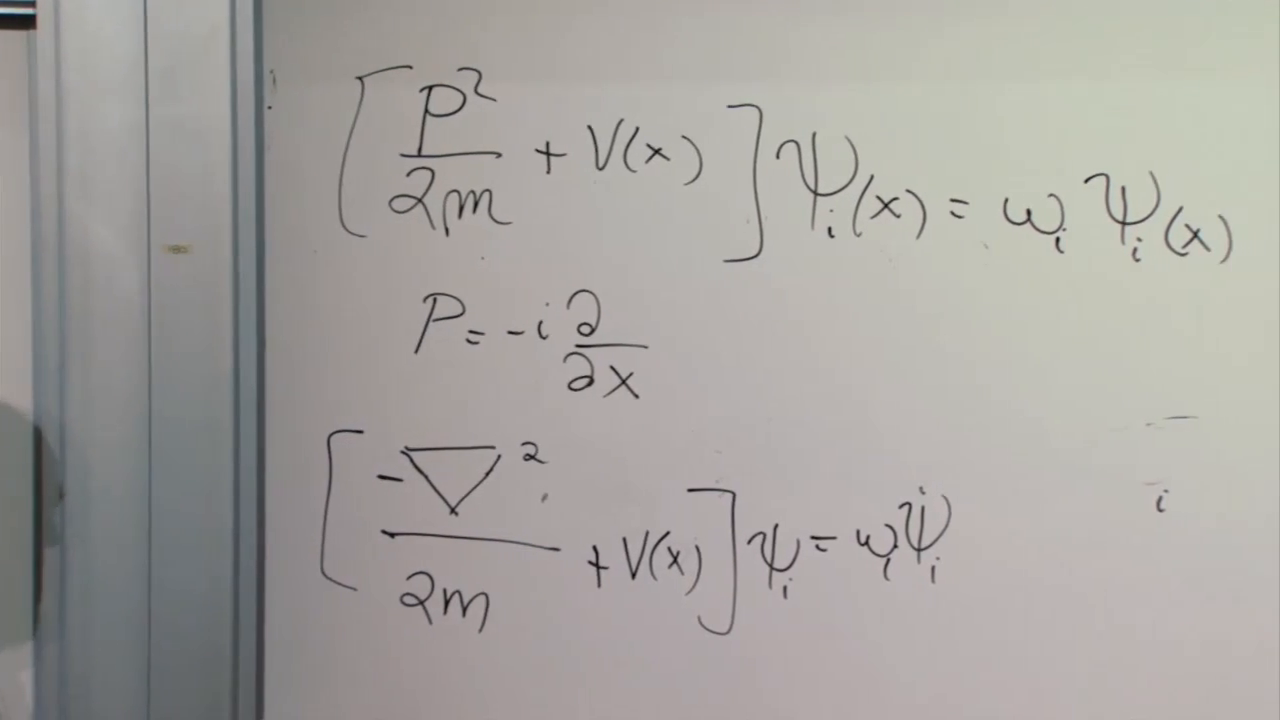
\includegraphics[width=0.94\linewidth]{lecture_07_frame_02.png}
\caption{Der Tafelabschnitt vom Ausdruck \(p^2/(2m)+V(x)\) bis zur Differentialform der Einteilchen-Schrödinger-Eigenwertgleichung. Gleichung~\eqref{eq:l07-schrodinger-eigenvalue} ist ihre bereinigte Rekonstruktion.}
\lectureframe{00:54:10}
\end{figure}

Für eine beliebige normierte Einteilchen-Wellenfunktion lautet der bekannte Erwartungswert
\begin{equation}
\langle h\rangle_\psi
=\int dx\,\psi^*(x)h\psi(x).
\label{eq:l07-one-particle-energy-expectation}
\end{equation}
Die Vielteilchenformel liegt nahe, wenn man die kleingeschriebene Wellenfunktion durch das operatorwertige Feld ersetzt. Das ist noch kein Beweis, sondern die Vermutung, deren Richtigkeit wir jetzt prüfen:
\begin{equation}
H=\int dx\,\Psi^\dagger(x)h\Psi(x).
\label{eq:l07-field-hamiltonian}
\end{equation}

\section{Zuerst die Antwort hinschreiben, dann beweisen}

Setzen wir Gleichung~\eqref{eq:l07-field-expansion} in den vorgeschlagenen Hamiltonoperator ein:
\begin{align}
\int dx\,\Psi^\dagger h\Psi
&=\int dx
\left(\sum_i a_i^\dagger\psi_i^*(x)\right)
h\left(\sum_j a_j\psi_j(x)\right) \\
&=\sum_{i,j}a_i^\dagger a_j
\int dx\,\psi_i^*(x)h\psi_j(x).
\label{eq:l07-h-expanded}
\end{align}
Der Differentialoperator \(h\) wirkt auf die von \(x\) abhängige Wellenfunktion \(\psi_j(x)\), nicht auf den Modenoperator \(a_j\). Nach der Schrödinger-Gleichung gilt
\begin{equation}
h\psi_j(x)=\omega_j\psi_j(x).
\end{equation}
Folglich
\begin{align}
\int dx\,\Psi^\dagger h\Psi
&=\sum_{i,j}a_i^\dagger a_j\omega_j
\int dx\,\psi_i^*(x)\psi_j(x) \\
&=\sum_{i,j}a_i^\dagger a_j\omega_j\delta_{ij} \\
&=\sum_j\omega_j a_j^\dagger a_j.
\label{eq:l07-h-proof}
\end{align}
Das ist genau Gleichung~\eqref{eq:l07-mode-hamiltonian}. Der lokale Feldausdruck und die Summe aller Teilchenenergien sind derselbe Operator.

\begin{figure}[htbp]
\centering
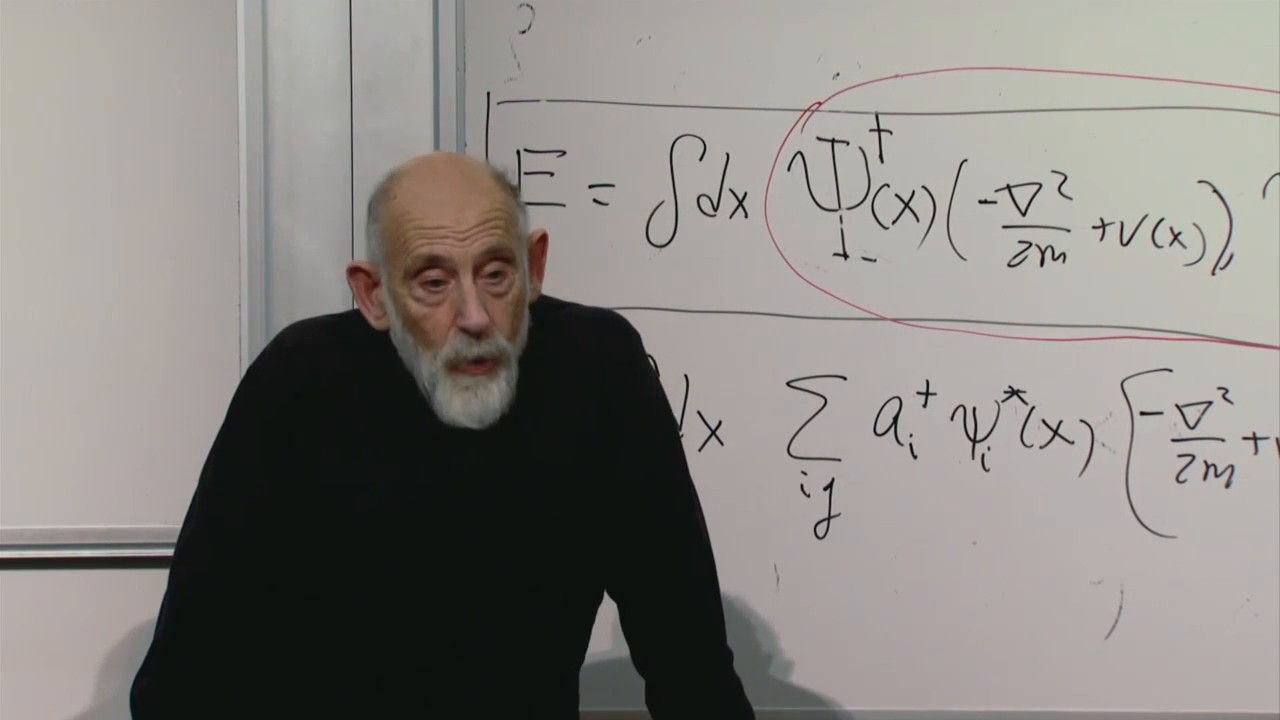
\includegraphics[width=0.94\linewidth]{lecture_07_frame_03.png}
\caption{Der an der Tafel hervorgehobene Feld-Hamiltonoperator; darunter beginnt der Beweis mit der Modenentwicklung. Der Live-Ausschnitt bleibt als Beleg erhalten; Gleichungen~\eqref{eq:l07-field-hamiltonian}--\eqref{eq:l07-h-proof} stellen die vollständige Rechnung wieder her.}
\lectureframe{01:05:34}
\end{figure}

Bei dieser Herleitung wurde kein Erzeugungsoperator an einem Vernichtungsoperator vorbeikommutiert. Die Reihenfolge \(a_i^\dagger a_j\) bleibt vom Anfang bis zum Ende erhalten. Nur die Wellenfunktionen und Eigenwerte, also \(c\)-Zahlen, werden frei verschoben.

\section{Warum ist das ein Feld?}

Warum nennen wir \(\Psi(x)\) ein Feld? Weil es eine operatorwertige Größe ist, die an jedem Raumpunkt definiert ist, und weil daraus gebildete hermitesche Kombinationen oder bilineare Ausdrücke lokale Observablen sind. Die Dichte \(n(x)\) und der weiter unten angegebene lokale Energieausdruck sind zwei Beispiele. Hinter dem Wort verbirgt sich kein zusätzliches mathematisches Kriterium.

Dieses Feld ist nicht das elektromagnetische Feld. Es beschreibt die nichtrelativistische Teilchensorte, deren Einteilchenmoden und Hamiltonoperator \(p^2/(2m)+V\) zugrunde gelegt wurden: beispielsweise langsam bewegte Atome, Neutronen, Protonen oder Elektronen. Diese Teilchen sind die Quanten des jeweils zugehörigen Feldes, in demselben strukturellen Sinn, in dem Photonen die Quanten des elektromagnetischen Feldes sind.

\begin{classroomqa}
\lecturetimestamp{01:02:45}
\audiencequestion{Wo ist beim Übergang vom Vielteilchensystem zur obigen Formel ein Feld ins Spiel gekommen?}
\lecturerresponse{In Gleichung~\eqref{eq:l07-field-expansion}: \(\Psi(x)\) ist ein Operator an jedem Raumpunkt. Die anschließenden Herleitungen zeigen, dass seine lokalen Produkte Teilchen- und Energiedichten messen. Ortsabhängigkeit zusammen mit Operatorcharakter ist genau die Feldstruktur, die wir konstruieren.}
\end{classroomqa}

\section{Lokale Energiedichte}

Gleichung~\eqref{eq:l07-field-hamiltonian} schreibt die Gesamtenergie als Integral über den Raum:
\begin{equation}
\begin{aligned}
H&=\int dx\,\mathcal H(x),\\
\mathcal H(x)
&=-\frac{1}{2m}\Psi^\dagger(x)\nabla^2\Psi(x)\\
&\quad+V(x)\Psi^\dagger(x)\Psi(x).
\end{aligned}
\label{eq:l07-hamiltonian-density}
\end{equation}
Der Integrand ist eine naheliegende lokale Energiedichte für diesen Hamiltonoperator. Ihre lokale Form ist nicht eindeutig. So ersetzt die partielle Integration den kinetischen Term durch
\begin{equation}
\mathcal H_{\rm kin}(x)
=\frac{1}{2m}\nabla\Psi^\dagger(x)\mathbin{\cdot}\nabla\Psi(x)
\label{eq:l07-kinetic-density}
\end{equation}
bis auf einen Randterm. Unter den üblichen Randbedingungen ergeben beide Ausdrücke denselben Gesamt-Hamiltonoperator. Das ist die kleine Mehrdeutigkeit, die in der Vorlesung erwähnt wurde.

\begin{classroomqa}
\lecturetimestamp{01:05:57}
\audiencequestion{Muss man die Energiedichte über den gesamten Raum integrieren?}
\lecturerresponse{Die Integration über den gesamten Raum ergibt die Gesamtenergie. Die Integration über ein kleineres Gebiet ergibt die diesem Gebiet zugeordnete Energie, wobei die gewöhnliche Mehrdeutigkeit bei der Wahl einer lokalen Dichte zu berücksichtigen ist, deren Integral über den ganzen Raum denselben Hamiltonoperator ergibt.}
\end{classroomqa}

\begin{classroomqa}
\lecturetimestamp{01:06:25}
\audiencequestion{Wie unterscheidet sich das großgeschriebene \(N_i\) in der Energieformel vom kleingeschriebenen \(n_i\)?}
\lecturerresponse{\(N_i=a_i^\dagger a_i\) ist ein Operator. Die ganze Zahl \(n_i\) ist einer seiner Eigenwerte auf einem Besetzungszahlzustand. Operatoren wirken auf Zustände; ihre Eigenwerte sind gewöhnliche Zahlen.}
\end{classroomqa}

\begin{classroomqa}
\lecturetimestamp{01:06:46}
\audiencequestion{Kann man den Feld-Hamiltonoperator selbst in Dirac-Notation als Bra oder Ket schreiben?}
\lecturerresponse{Nein. Bras und Kets bezeichnen Zustandsvektoren und ihre Dualvektoren. Das Feld und der Hamiltonoperator sind Operatoren, die auf diese Zustände wirken. Ein Erwartungswert wie \(\langle\Phi|H|\Phi\rangle\) verwendet beide Arten von Objekten; man darf sie nicht gleichsetzen.}
\end{classroomqa}

\section{Ein Teilchen zurückgewinnen und sich einem klassischen Feld nähern}

Der erweiterte Formalismus enthält die gewöhnliche Einteilchen-Quantenmechanik. Beschränken wir den Fockraum auf Zustände, für die
\begin{equation}
N|\Phi\rangle=|\Phi\rangle.
\end{equation}
gilt. Innerhalb dieses Sektors reproduziert die Feldkonstruktion jeden Einteilchenzustand und jede Einteilchenvorhersage. Wir haben die alte Theorie nicht ersetzt, sondern sie in einen Raum eingebettet, der auch null, zwei oder beliebig viele Teilchen beschreiben kann.

Am anderen Ende kann sich eine Mode, die von sehr vielen Bosonen besetzt ist, näherungsweise wie eine klassische Welle verhalten. In geeigneten kohärenten oder semiklassischen Zuständen erfüllt der Erwartungswert
\begin{equation}
\Phi_{\rm cl}(x,t)=\langle\Psi(x,t)\rangle
\end{equation}
die klassisch anmutende Gleichung
\begin{equation}
i\partial_t\Phi_{\rm cl}(x,t)
=\left(-\frac{\nabla^2}{2m}+V(x)\right)\Phi_{\rm cl}(x,t)
\label{eq:l07-classical-schrodinger}
\end{equation}
für die freie nichtrelativistische Theorie. Die Vorlesung stellt diesen Zusammenhang dar, ohne ihn herzuleiten. Er bildet die Brücke zwischen einer Ansammlung von Quanten und einem Wellenfeld: Bei großer Besetzung werden die relativen Fluktuationen klein, sodass sich geeignete Erwartungswerte klassisch verhalten.

Der Formalismus ist also zugleich Buchführung und Physik. Er ordnet alle Teilchenzahlsektoren, erfasst aber auch Interferenz, Verschränkung und das Entstehen klassischer Wellen aus Quantenteilchen.

\begin{classroomqa}
\lecturetimestamp{01:10:43}
\audiencequestion{Warum lassen sich die Erzeugungs- und Vernichtungsoperatoren im Integral beinahe wie gewöhnliche Zahlen behandeln?}
\lecturerresponse{Sie wurden nie miteinander vertauscht. Die gewöhnlichen Modenfunktionen kommutieren mit ihnen, und die Ableitungen wirken nur auf diese Funktionen. Einen Vernichtungsoperator an einem Erzeugungsoperator vorbeizuziehen, würde den Kommutator erfordern und könnte einen zusätzlichen Term ergeben; in der Herleitung wird dieser Schritt nicht ausgeführt.}
\end{classroomqa}

\section{Ein Einschub zur Dirac-Notation}

Ein Teil der Verwirrung ist historisch bedingt. Eine Einteilchen-Wellenfunktion erfüllt eine Wellengleichung und sieht oberflächlich wie ein klassisches Feld aus, ist zugleich aber eine Wahrscheinlichkeitsamplitude. Die frühe Quantentheorie musste diese Rollen auseinanderhalten und anschließend erklären, wie echte messbare Wellenfelder wie das elektromagnetische Feld aus Quanten aufgebaut sind. Fockraum und operatorwertige Felder lösen den scheinbaren Widerspruch auf.

Die Dirac-Notation fasst diese Unterscheidung besonders knapp. Ein Ket gehört zu einem Vektorraum, ein Bra zu seinem Dualraum, und ihre Nebeneinanderschreibung bildet ein Skalarprodukt. Die Vollständigkeitsrelation
\begin{equation}
\sum_i|i\rangle\langle i|=\mathbf 1
\end{equation}
wird damit beinahe selbsterklärend. Die Vorlesung veranschaulicht dies anhand einer Anekdote aus dem Quantenmechanikunterricht für Mathematiker: Der mathematische Inhalt war bereits vertraut, doch die Notation machte routinemäßige Umformungen so durchsichtig, dass die Struktur neu erschien. Es geht nicht darum, dass einer Fachrichtung der Begriff fehlte. Eine gut gewählte Notation kann vielmehr dafür sorgen, dass die zulässigen Operationen kaum zu verwechseln sind.

Das ist hier wichtig. Es gibt nun mehrere verschiedene Operatoren:
\begin{itemize}
\item \(h\) wirkt als Differentialoperator auf Einteilchen-Wellenfunktionen;
\item \(a_i\) und \(a_i^\dagger\) wirken auf Besetzungszahlzustände im Fockraum;
\item \(\Psi(x)\), \(\Psi^\dagger(x)\), \(N\) und \(H\) wirken ebenfalls auf den Fockraum.
\end{itemize}
Die Entwicklung in Gleichung~\eqref{eq:l07-field-expansion} verknüpft die ersten beiden Bereiche, ohne sie miteinander zu verschmelzen.

\begin{classroomqa}
\lecturetimestamp{01:18:16}
\audiencequestion{Sind Felder nur ein Formalismus zur Beschreibung von Teilchensammlungen?}
\lecturerresponse{Sie sind ein Formalismus, aber kein inhaltsleerer. Ihre lokalen Observablen lassen sich messen, und die Teilchen sind Quantenobjekte mit Interferenz und Verschränkung, keine klassischen Kügelchen. Die Feldoperatoren kodieren genau diese messbaren kollektiven Eigenschaften.}
\end{classroomqa}

\section{Relativistische Vorsicht und ein Exkurs zum Elektromagnetismus}

Die bisherige Konstruktion ist nichtrelativistisch. Der Impuls bleibt in der relativistischen Physik eine gute Teilchenbezeichnung, doch die scharfe Lokalisierung eines Teilchens am Ort ist wesentlich problematischer. Daher ist eine lokale Photonenzahldichte im Allgemeinen kein so klar definierter Gegenstand wie die nichtrelativistische Dichte \(n(x)\). Die Energiedichte bleibt wohldefiniert und ist die sicherere lokale Observable.

Die Vorlesung führt eine nützliche, ausdrücklich heuristische Analogie zum Elektromagnetismus an. Man fasse das elektrische und das magnetische Feld zum komplexen Vektor
\begin{equation}
\mathbf F=\mathbf E+i\mathbf B,
\qquad
\mathbf F^*=\mathbf E-i\mathbf B.
\label{eq:l07-riemann-silberstein}
\end{equation}
zusammen. Dann gilt
\begin{equation}
\mathbf F^*\mathbin{\cdot}\mathbf F
=\mathbf E^2+\mathbf B^2,
\label{eq:l07-em-density}
\end{equation}
was in konventionellen Einheiten proportional zur elektromagnetischen Energiedichte ist. Das ist nicht wörtlich eine Photon-Wahrscheinlichkeitsdichte. Treffender ist es, diese Größe als kompakte Feldvariable zu verstehen, deren Betragsquadrat die Energiedichte misst, oder informell als Photonendichte, gewichtet mit der Photonenenergie.

\begin{classroomqa}
\lecturetimestamp{01:19:10}
\audiencequestion{Kann man die Photonendichte mit der Stärke des elektrischen Feldes gleichsetzen?}
\lecturerresponse{Nur qualitativ und mit Vorsicht. Für relativistische Photonen ist die lokale Teilchenzahl nicht der bevorzugte Begriff. Die belastbare Aussage ist, dass \(E^2+B^2\) proportional zur Energiedichte ist und dass die komplexe Kombination \(\mathbf E+i\mathbf B\) die Maxwell-Gleichungen in einer Schrödinger-ähnlichen Form zusammenfasst.}
\end{classroomqa}

\begin{classroomqa}
\lecturetimestamp{01:20:09}
\audiencequestion{Warum kann ein relativistisches Teilchen einen bestimmten Impuls haben, während sein Ort problematisch ist?}
\lecturerresponse{Der Impuls kennzeichnet relativistische Einteilchen-Darstellungen eindeutig, wohingegen eine strikte Lokalisierung mit der Teilchenerzeugung und der relativistischen Feldbeschreibung in Konflikt gerät. Diese Vorlesung entwickelt jene Theorie nicht; der Hinweis markiert die Grenze der hier behandelten nichtrelativistischen Deutung der Dichte.}
\end{classroomqa}

\section{Operatorordnung und die Grundzustandskonstante}

Die Operatorreihenfolge darf nicht leichtfertig geändert werden. Für bosonische Moden gilt
\begin{equation}
a_i a_i^\dagger=a_i^\dagger a_i+1.
\end{equation}
Ersetzt man daher die Normalordnung \(\Psi^\dagger h\Psi\) durch die umgekehrte Reihenfolge \((h\Psi)\Psi^\dagger\) oder die entsprechende integrierte Form, kommt der Kommutatorbeitrag hinzu. In einer Modenbasis ist dies eine additive Summe von einer Energiequant pro Mode. Es handelt sich um die Grundzustands- oder Nullpunktskonstante, die im Kontinuum regularisiert werden muss. Die Vorlesung geht diesem Problem hier nicht weiter nach; sie weist lediglich darauf hin, dass die beiden Anordnungen nicht gleich sind.

\begin{classroomqa}
\lecturetimestamp{01:22:04}
\audiencequestion{Was geschieht, wenn \(\Psi\) und \(\Psi^\dagger\) im Hamiltonoperator vertauscht werden?}
\lecturerresponse{Ihr Kommutator muss berücksichtigt werden. Beim Umkehren der Reihenfolge kommt daher ein zustandsunabhängiger Grundzustandsbeitrag hinzu, statt dass derselbe Ausdruck entsteht. Der angegebene Hamiltonoperator steht in Normalordnung, \(\Psi^\dagger h\Psi\).}
\end{classroomqa}

\section{Der Impuls als letzter Test}

In den letzten Minuten wird dieselbe Ersetzung noch einmal vorgenommen. Für ein Teilchen gilt
\begin{equation}
\langle p\rangle_\psi
=\int dx\,\psi^*(x)\left(-i\partial_x\right)\psi(x).
\label{eq:l07-one-particle-momentum}
\end{equation}
Ersetzt man die Wellenfunktion durch das Feld, erhält man den Operator des Gesamtimpulses
\begin{equation}
P=\int dx\,\Psi^\dagger(x)\left(-i\partial_x\right)\Psi(x),
\label{eq:l07-field-momentum}
\end{equation}
oder in drei Dimensionen
\begin{equation}
\mathbf P=\int d^3x\,\Psi^\dagger(\mathbf x)
\left(-i\boldsymbol\nabla\right)\Psi(\mathbf x).
\end{equation}
Felder tragen Impuls. Ein hinreichend leistungsstarker Laser überträgt Impuls auf eine Wand und übt eine Kraft auf sie aus; in der quantenmechanischen Beschreibung ist dieser Feldimpuls die Summe der Impulse der Photonen.

Gleichung~\eqref{eq:l07-field-momentum} gibt einen Operator an, keinen Erwartungswert. Für einen Fock-Raum-Zustand \(|\Phi\rangle\) kann man dann berechnen
\begin{equation}
\langle P\rangle_\Phi=\langle\Phi|P|\Phi\rangle.
\end{equation}
Für die Bildung eines Erwartungswerts sind sowohl ein Operator als auch ein Zustand erforderlich. Wer die Observable mit ihrem Mittelwert verwechselt, verwischt genau den Unterschied, den diese Vorlesung herausgearbeitet hat.

\begin{classroomqa}
\lecturetimestamp{01:26:02}
\audiencequestion{Ist der angegebene Feldimpuls bereits der mittlere Impuls?}
\lecturerresponse{Nein. Er ist der hermitesche Operator, der die Observable darstellt. Gibt man einen Zustand vor, erhält man den Erwartungswert, indem man den Operator zwischen dessen Bra und Ket einfasst; bei einer Messung kann der Messwert weiterhin um diesen Mittelwert schwanken.}
\end{classroomqa}

Dies ist ein natürlicher Schlusspunkt. Ausgehend von Teilchen haben wir lokale Erzeugungs- und Vernichtungsfelder konstruiert, sie zum Zählen von Teilchen verwendet und die Summe der Einteilchenenergien und -impulse als Feldoperatoren umgeschrieben. Der nächste Schritt ist keine weitere Änderung der Schreibweise. Nun sollen Feldoperatoren physikalische Prozesse darstellen: Teilchen zerfallen, Teilchen streuen und Teilchensorten ineinander umgewandelt werden.